\section{检验结果}

在了解了相关的视图知识后,让我们来简单地检验下套筒零件的三维模型的投影是不是与零件图的视图基本一致的。为什么说是基本一致呢,主要是因为接下来的检验方法仅仅是在AutoCAD的模型空间中,用切换视图方向的方法进行观察套筒的三维模型,其表现方式类似于生活中的影子,并不符合工程图的制图规范。

\begin{procedure}
\item 将视觉样式切换为二维线框

在\ref{sec:taotongjianmo}节中,为了便于看到真实的套筒零件三维模型,我们将视觉样式设置成了灰度。在本节中为了方便观察不同方向的视图,我们需要将视觉样式设置为二维线框方式。

\begin{lstlisting}
命令: VSCURRENT
输入选项 [二维线框(2)/线框(W)/隐藏(H)/真实(R)/概念(C)/着色(S)/带边缘着色(E)/灰度(G)/勾画(SK)/X 射线(X)/其他(O)] <灰度>: 2
\end{lstlisting}
\item 观察主视图

要观察套筒的主视图,需要将三维视图切换为前视图方向,其切换方法与\ref{sec:taotongjianmo}节中切换左视图的方法基本相同,图\ref{fig:taotongfront} 所示为切换为前视图后的结果。从图中可以看出,整个图形的外形与套筒零件的主视图外形是一致的,主要区别是关于内部结构的表达。

\begin{lstlisting}
命令: -VIEW
输入选项 [?/删除(D)/正交(O)/恢复(R)/保存(S)/设置(E)/窗口(W)]: front
\end{lstlisting}
\item 观察左视图

将视图方向切换为左视图,可以得到图\ref{fig:taotongleft}所示的结果。从图中可以看出,他与套筒的左视图是基本相同。
\begin{lstlisting}
命令: -VIEW
输入选项 [?/删除(D)/正交(O)/恢复(R)/保存(S)/设置(E)/窗口(W)]: left
\end{lstlisting}
\item 观察俯视图

将视图切换为俯视图后,其结果如图\ref{fig:taotongtop}所示,可以看它与主视图方向的一图形是一致的。
\begin{lstlisting}
命令: -VIEW
输入选项 [?/删除(D)/正交(O)/恢复(R)/保存(S)/设置(E)/窗口(W)]: top
\end{lstlisting}
\begin{figure}[htbp]
\subfloat[主视图]{\label{fig:taotongfront}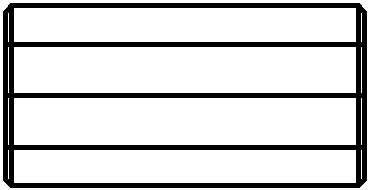
\includegraphics[scale=0.5]{taotongfront.png}}\hspace{15pt}
\subfloat[左视图]{\label{fig:taotongleft}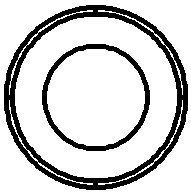
\includegraphics[scale=0.5]{taotongleft.png}}\hspace{15pt}
\subfloat[俯视图]{\label{fig:taotongtop}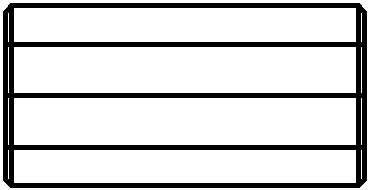
\includegraphics[scale=0.5]{taotongfront.png}}
\end{figure}
\end{procedure}

从上面的简单检验结果来看,我们套筒零件的三维建模是正确。其实,这种简单的检验方法将在AutoCAD的建模过程中会经常用到,尽管他与实际工作图存在一定的差别,但是它的操作步骤简便,能够快速地验证结果,能够有效地辅助三维建模,比较实用。
\endinput